\documentclass{beamer}
\usepackage{algorithm}
\usepackage{algpseudocode}
\usepackage{graphicx}

\usetheme{Madrid}
\usecolortheme{default}

\title{Metodi del Calcolo Scientifico}
\subtitle{Progetto 1 Bis}
\author{Francesco~Refolli.~865955}
%\logo{
\includegraphics[height=1cm]{logo_unimib.pdf}}

\newcommand{\putimagecouple}[4] {
  \begin{figure}[!htb]
      \centering
      \begin{minipage}{0.45\linewidth}
          \centering
          \includegraphics[width=\linewidth]{#1}
          \caption{#2}
      \end{minipage}
      \hspace{0.25cm}
      \begin{minipage}{0.45\linewidth}
          \centering
          \includegraphics[width=\linewidth]{#3}
          \caption{#4}
      \end{minipage}
  \end{figure}
}

\begin{document}

\frame{\titlepage}

\begin{frame}
\frametitle{Indice}
\tableofcontents
\end{frame}

\section{Introduzione}

\begin{frame}
\frametitle{Introduzione}

Implementazione di alcuni \textbf{metodi iterativi}:
\begin{itemize}
  \item metodo di Jacobi
  \item metodo di Gauss-Seidel
  \item metodo del Gradiente
  \item metodo del Gradiente Coniugato
\end{itemize}

e alcuni \textbf{metodi diretti}:
\begin{itemize}
  \item sostituzione in avanti
  \item sostituzione all'indietro
\end{itemize}

\begin{figure}
  \centering
  
\includegraphics[height=1cm]{images/cpp.png}
  \hspace{0.5cm}
  
\includegraphics[height=1cm]{images/eigen.png}
  \hspace{0.5cm}
  
\includegraphics[height=1cm]{images/spectra.png}
\end{figure}

\end{frame}

\section{Libreria}

\begin{frame}
\frametitle{Jacobi Engine}
\begin{figure}
  \centering
  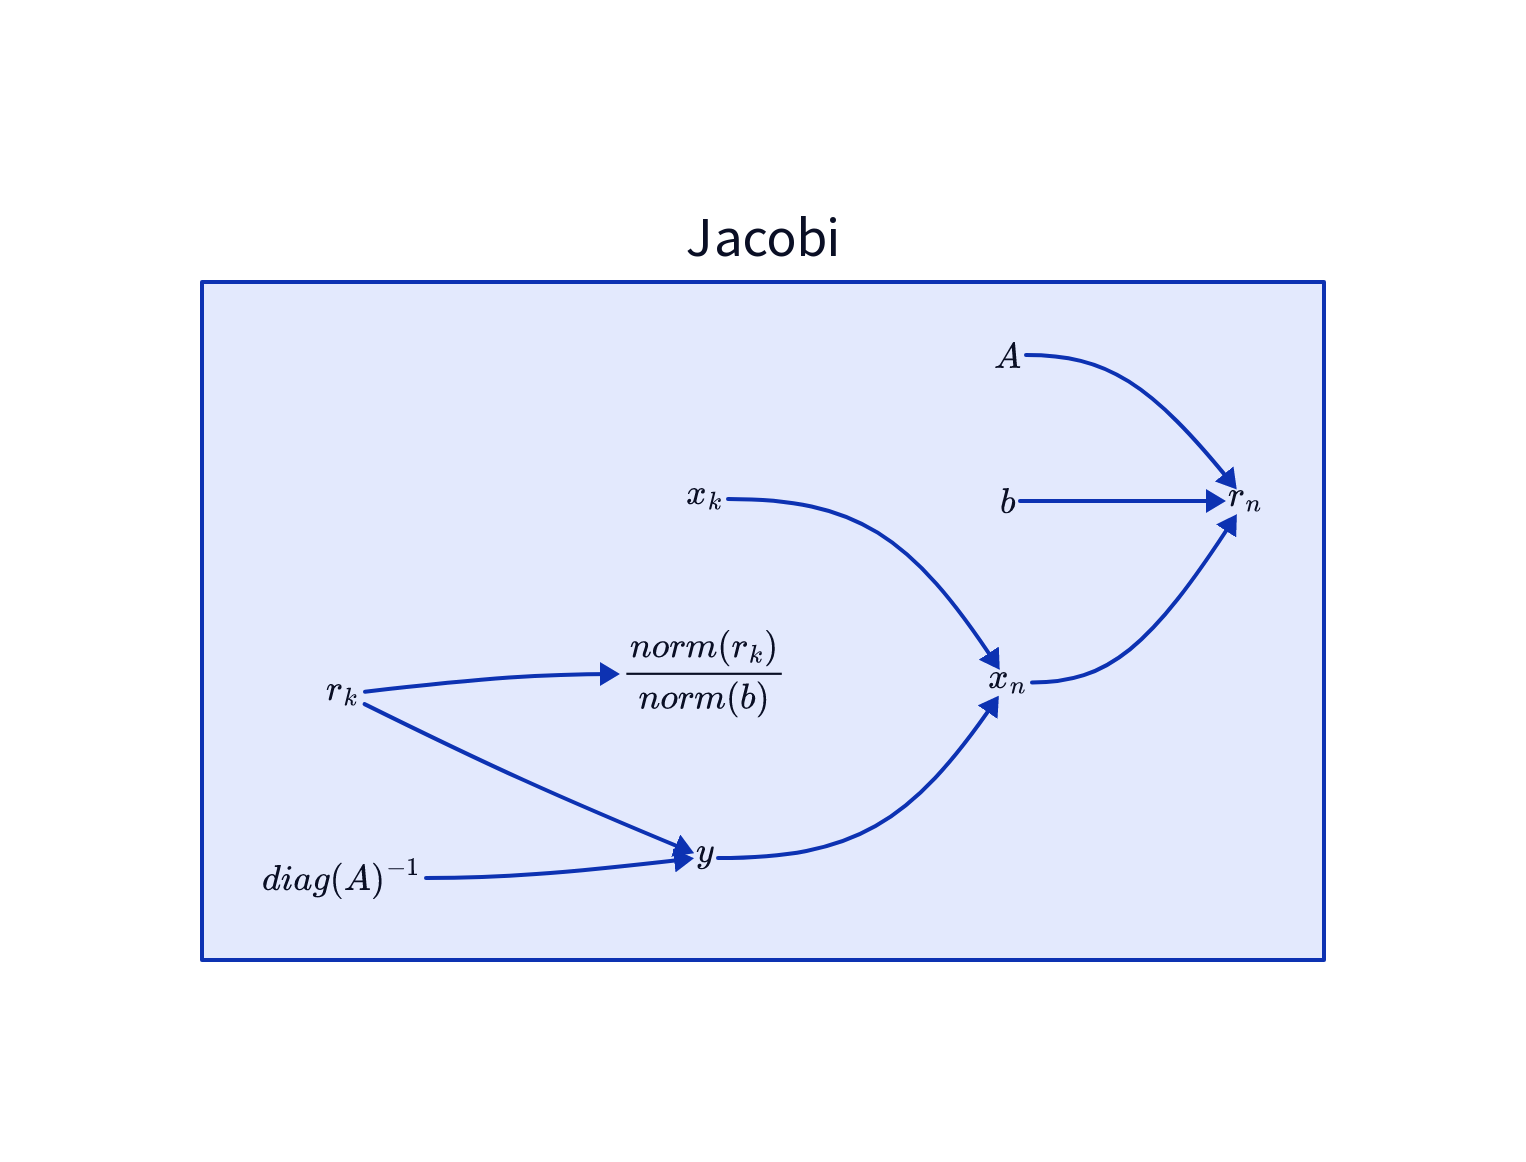
\includegraphics[width=\linewidth]{images/cd-jae.png}
\end{figure}
\end{frame}

\begin{frame}
\frametitle{Gauss-Seidel Engine}
\begin{figure}
  \centering
  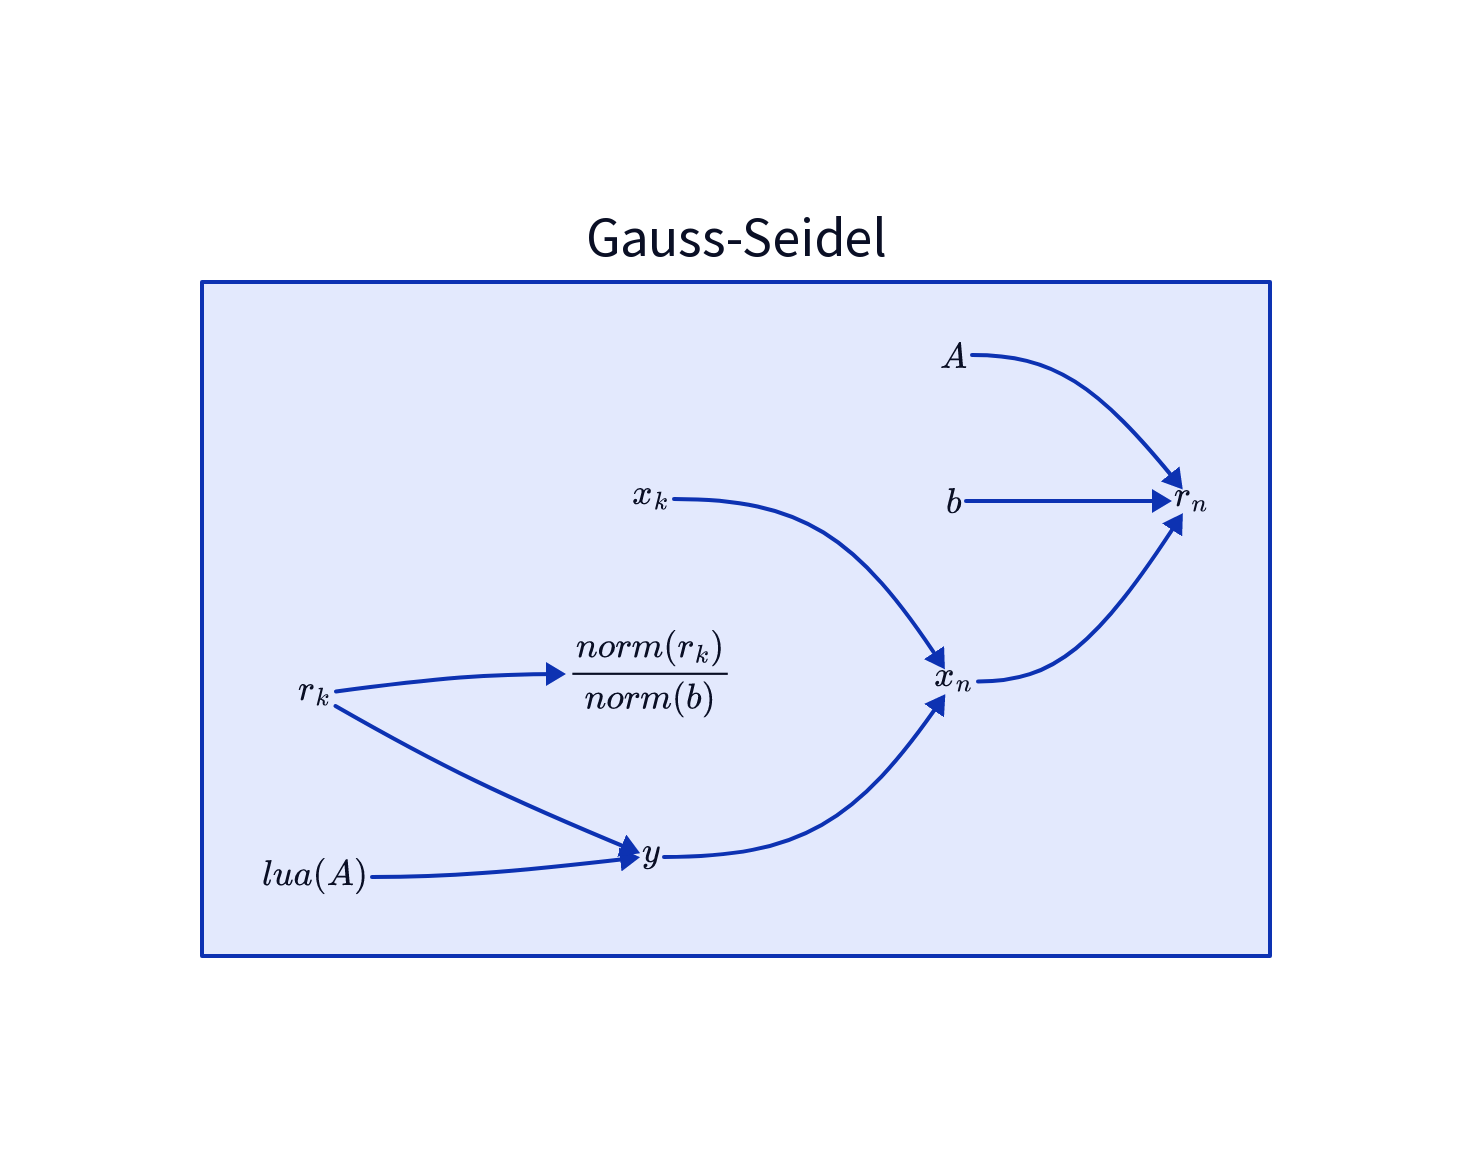
\includegraphics[width=\linewidth]{images/cd-gse.png}
\end{figure}
\end{frame}

\begin{frame}
\frametitle{Gradient Engine}
\begin{figure}
  \centering
  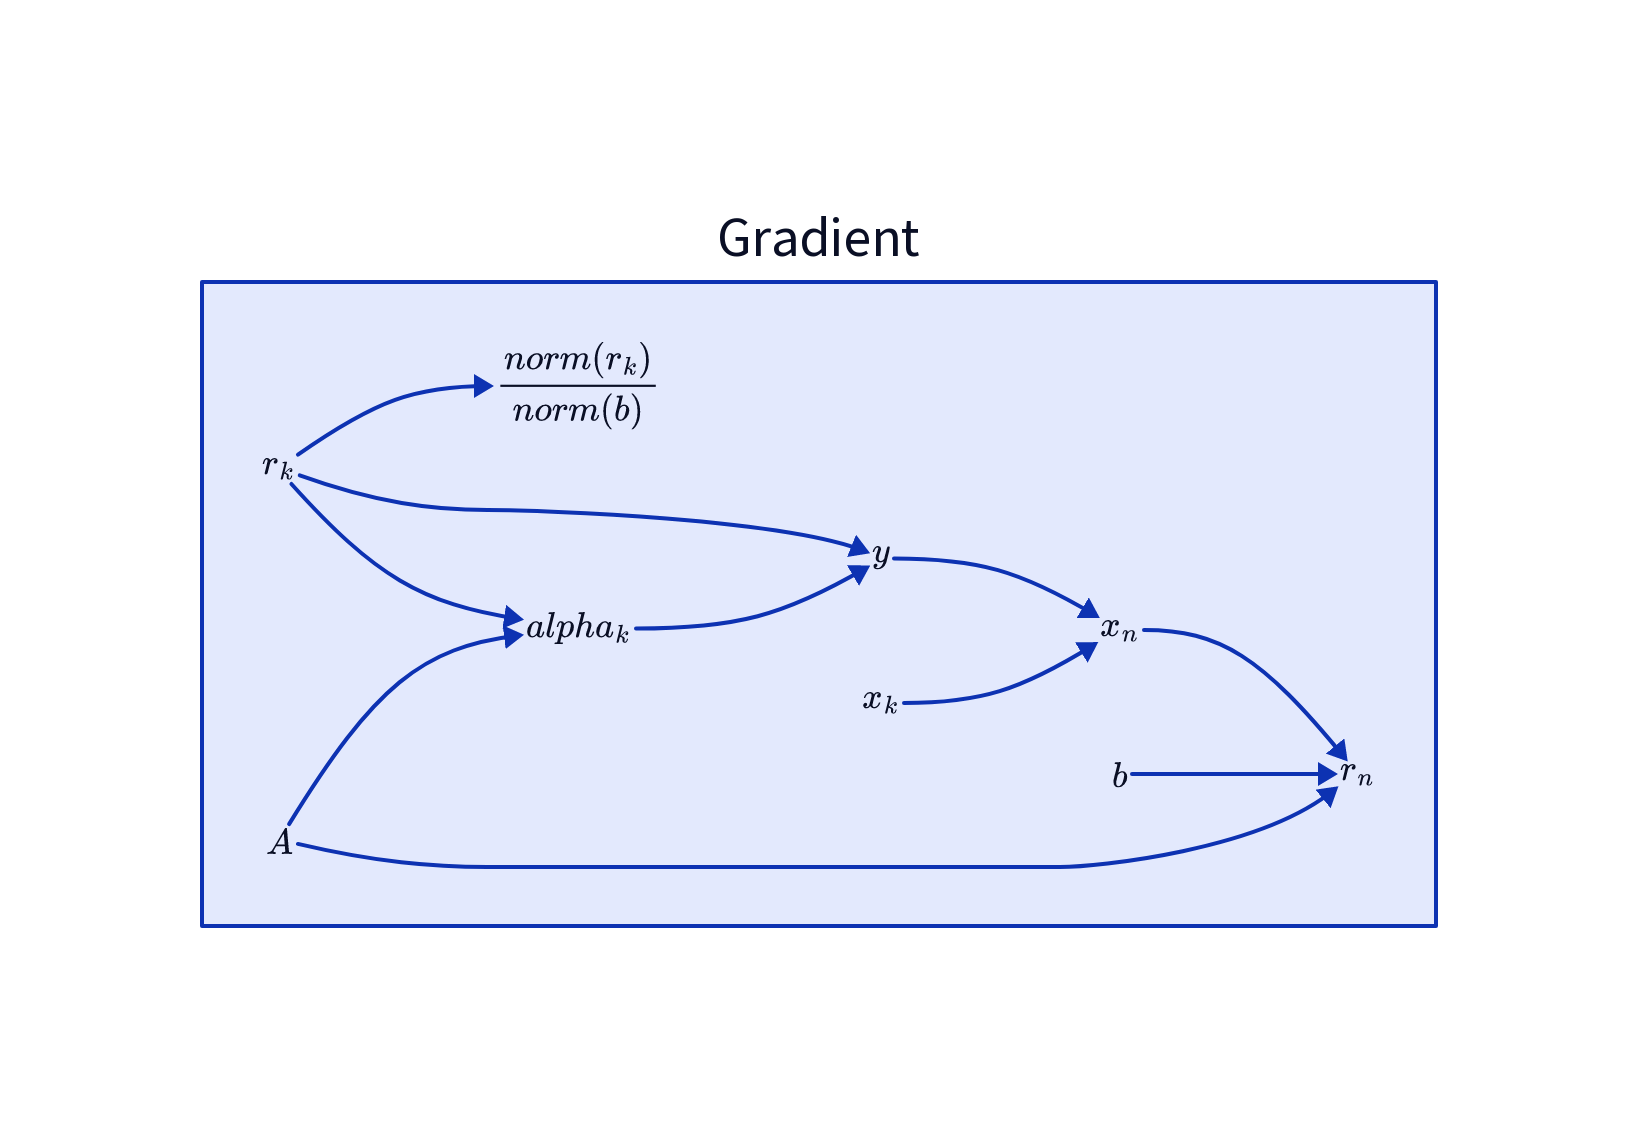
\includegraphics[width=\linewidth]{images/cd-gre.png}
\end{figure}
\end{frame}

\begin{frame}
\frametitle{Coniugate Gradient Engine}
\begin{figure}
  \centering
  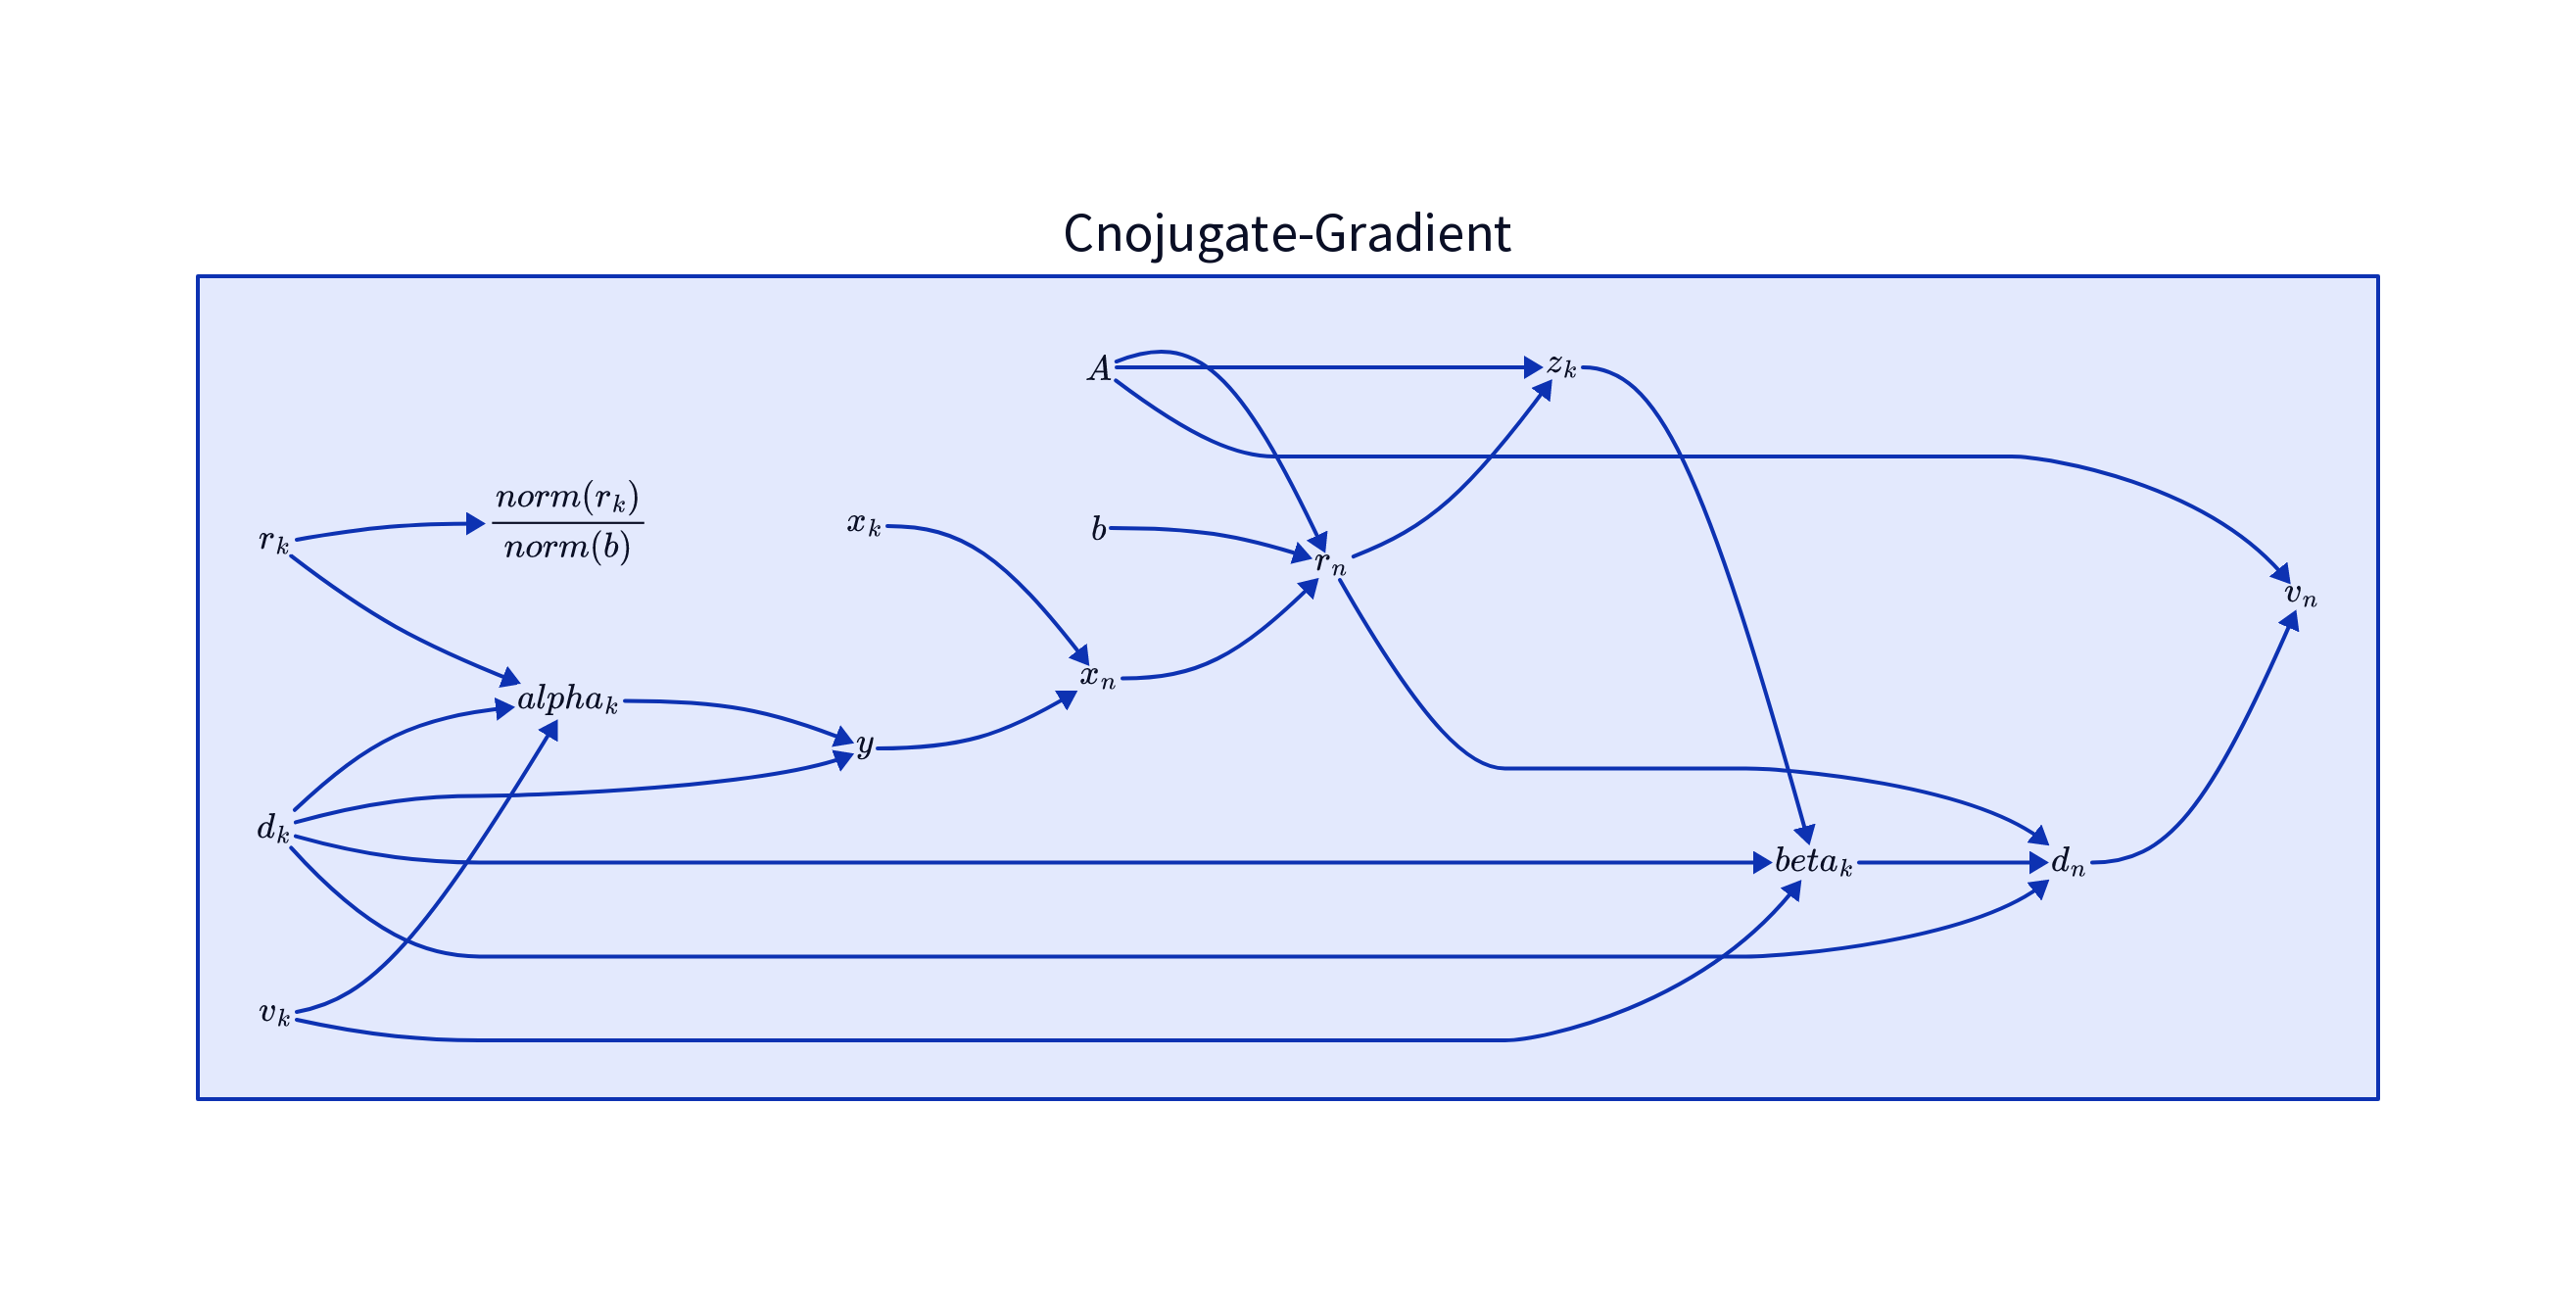
\includegraphics[width=\linewidth]{images/cd-cge.png}
\end{figure}
\end{frame}

\begin{frame}
\frametitle{Algoritmo Generale}
  \begin{center}
    \scalebox{0.67}{ % Adjust the scaling factor as needed
        \begin{minipage}{\textwidth} % This ensures proper grouping
          \begin{algorithm}[H]
          \renewcommand\thealgorithm{}
          \caption{Algoritmo Generale Iterativo}
          \begin{algorithmic}
            \Procedure{IterativeSolver::run}{$A, b, tol, maxIter$}
              \State $state \gets State::new()$
              \State $state.A \gets A$
              \State $state.b \gets b$
              \State $norm\_of\_b \gets state.b.norm()$
              \State $state.x_k \gets ArrayOfZeros(state.A.cols())$
              \State $state.r_k \gets state.b - state.A \cdot state.x_k$
              \State engine.post\_initialize(state)
              \For{$k \gets 1$ to $maxIter$}
                \State $normalized\_residual \gets \frac {state.r_k.norm()} {norm\_of\_b}$
                \If{$normalized\_residual < tol$}
                  \State \Return $Ok(state.r_k)$
                \EndIf
                \State engine.pre\_compute\_y(state)
                \State engine.compute\_y(state)
                \State $state.x_n = state.x_k + state.y$
                \State $state.r_n \gets state.b - state.A \cdot state.x_n$
                \State engine.post\_compute\_x(state)
                \State state.update()
              \EndFor
              \State \Return $Err()$
            \EndProcedure
          \end{algorithmic}
        \end{algorithm}
        \end{minipage}
    }
  \end{center}
\end{frame}

\begin{frame}
\frametitle{Architetture}
\begin{figure}
  \centering
  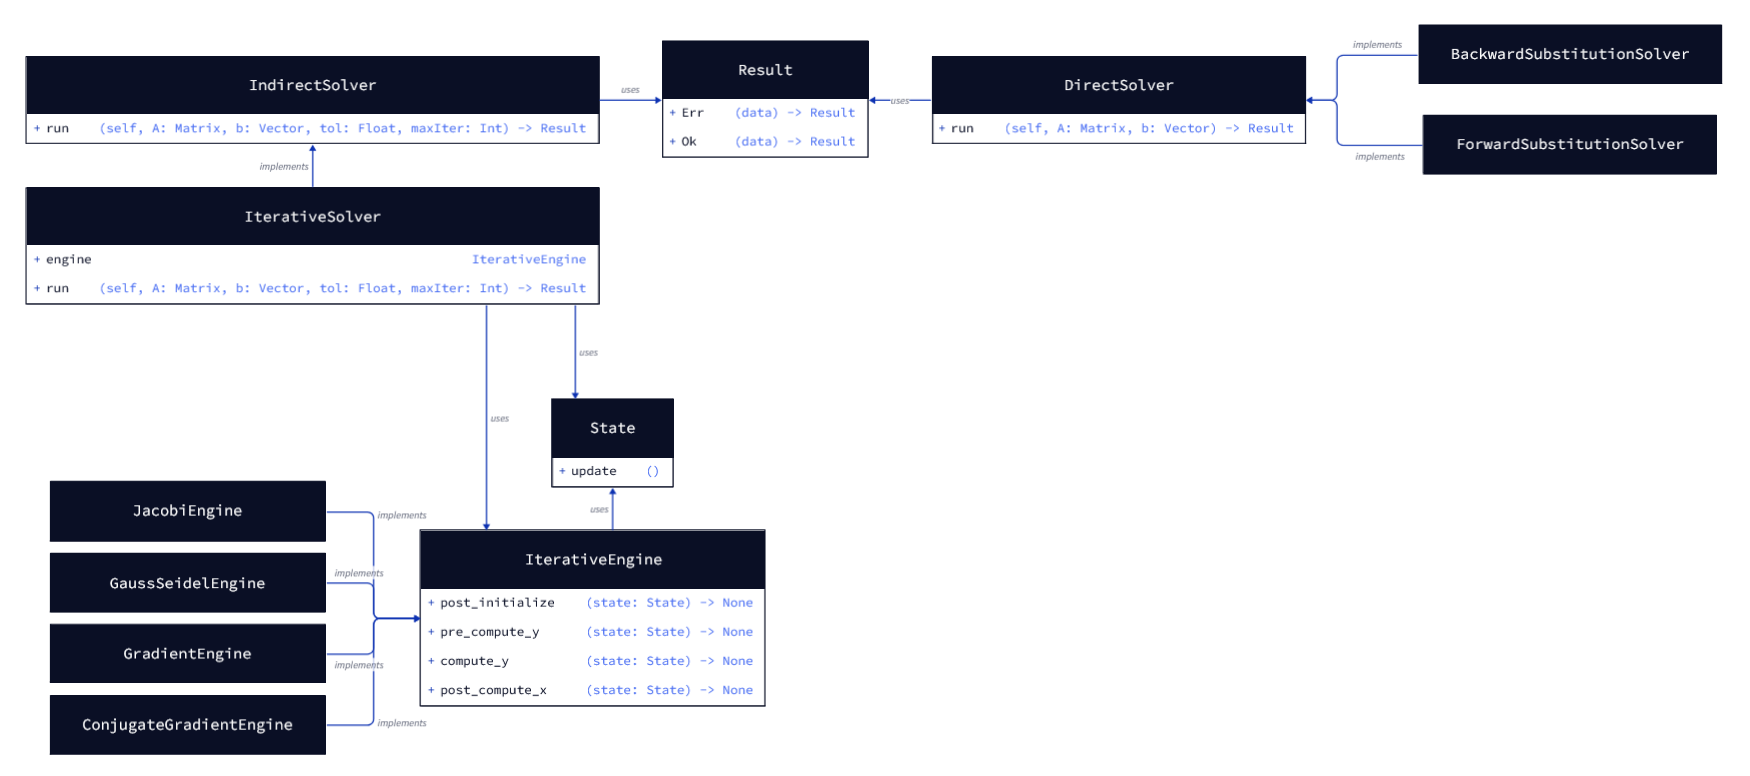
\includegraphics[width=\linewidth]{images/diagram.png}
\end{figure}
\end{frame}


\section{Matrici}

\begin{frame}
\frametitle{MatSpy di Spa1/2}
\putimagecouple{images/spy-spa1.png}{Spa1.mtx}{images/spy-spa2.png}{Spa2.mtx}
\end{frame}

\begin{frame}
\frametitle{MatSpy di Vem1/2}
\putimagecouple{images/spy-vem1.png}{Vem1.mtx}{images/spy-vem2.png}{Vem2.mtx}
\end{frame}

\begin{frame}
\frametitle{Plot della dominanza diagonale}
\begin{figure}
  \centering
  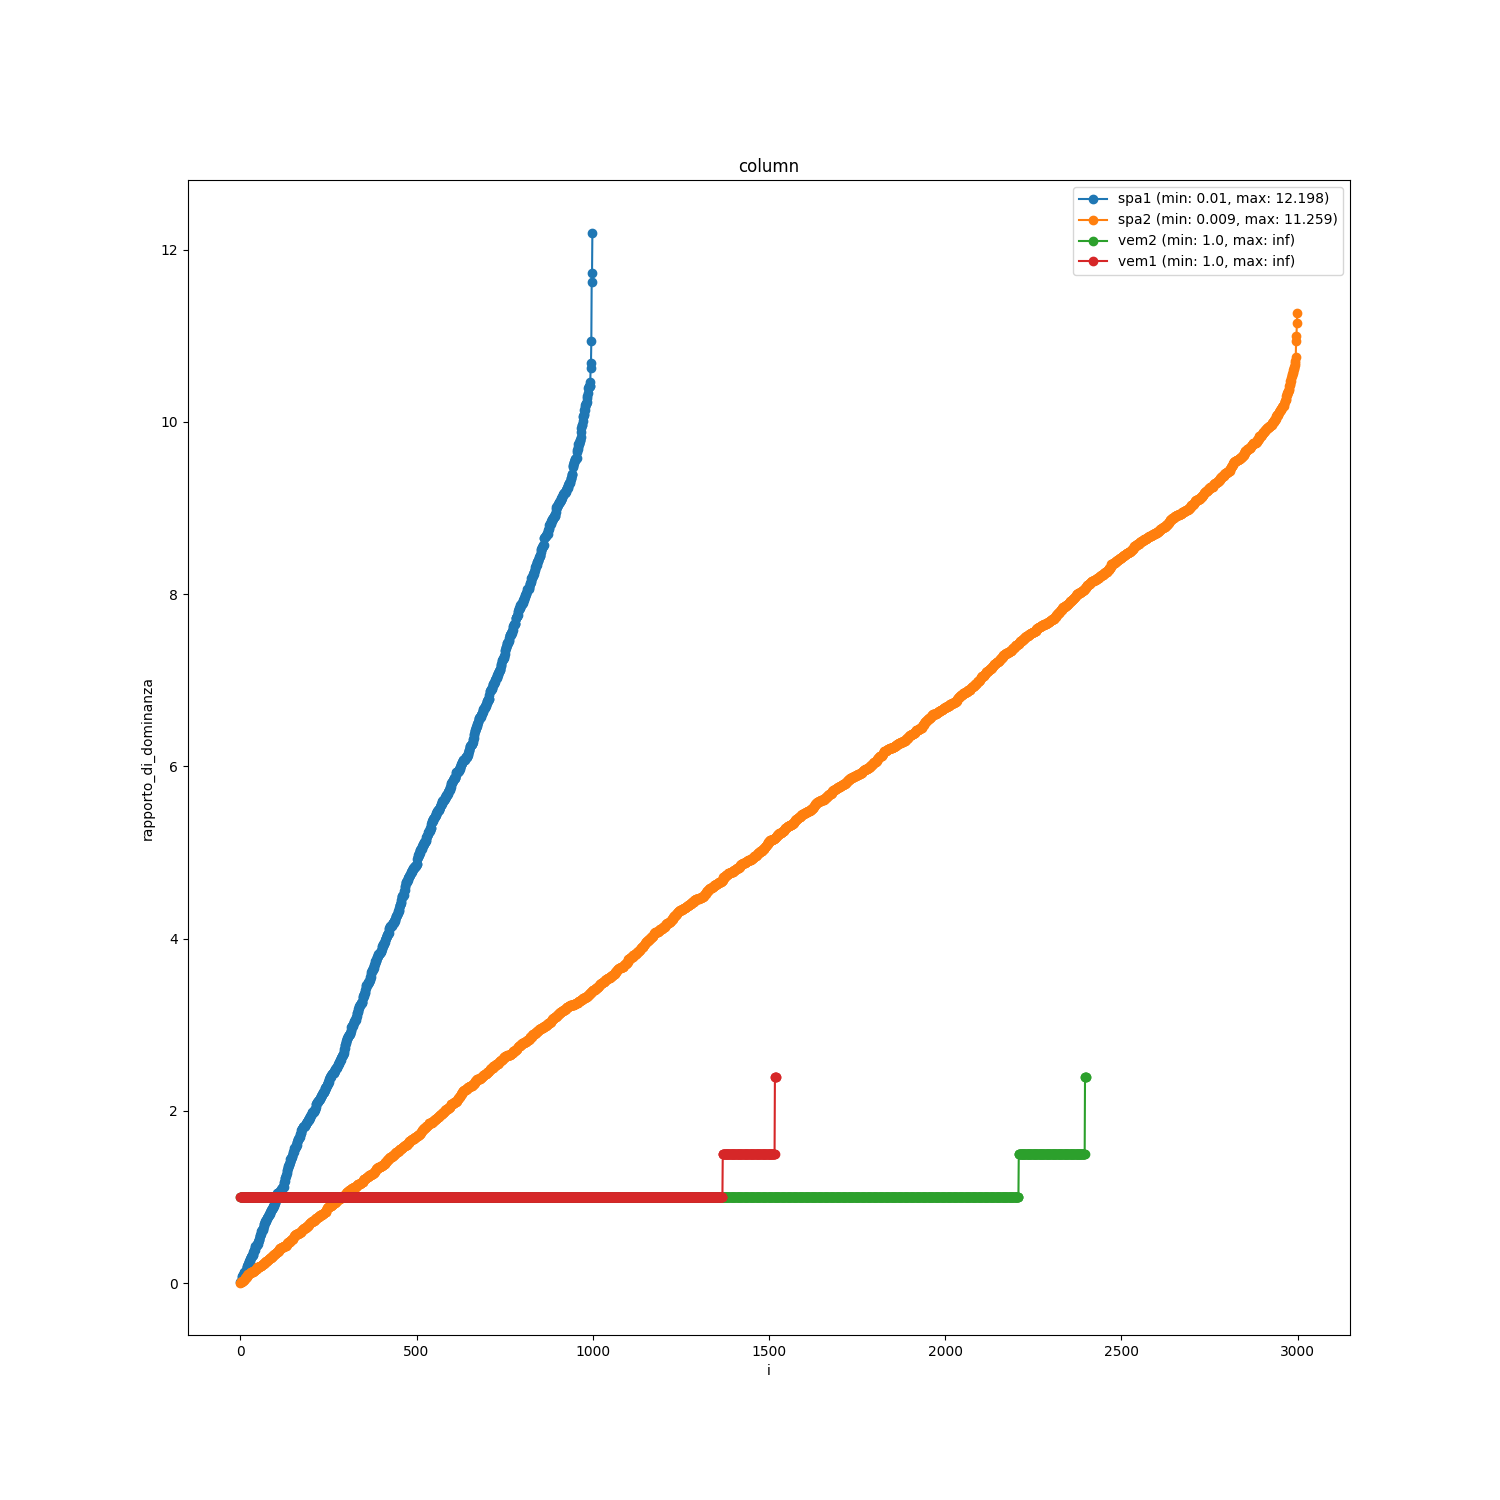
\includegraphics[width=0.7\linewidth]{images/dominance.png}
\end{figure}
\end{frame}

\section{Esperimenti}

\begin{frame}
\frametitle{Convergenza - Jacobi Engine}
\putimagecouple{images/it-re-jae.png}{Iterazioni $\times$ Residuo}{images/te-re-jae.png}{Tempo $\times$ Residuo}
\end{frame}

\begin{frame}
\frametitle{Convergenza - Gauss-Seidel Engine}
\putimagecouple{images/it-re-gse.png}{Iterazioni $\times$ Residuo}{images/te-re-gse.png}{Tempo $\times$ Residuo}
\end{frame}

\begin{frame}
\frametitle{Convergenza - Gradient Engine}
\putimagecouple{images/it-re-gre.png}{Iterazioni $\times$ Residuo}{images/te-re-gre.png}{Tempo $\times$ Residuo}
\end{frame}

\begin{frame}
\frametitle{Convergenza - Coniugate Gradient Engine}
\putimagecouple{images/it-re-cge.png}{Iterazioni $\times$ Residuo}{images/te-re-cge.png}{Tempo $\times$ Residuo}
\end{frame}

\begin{frame}
\frametitle{Scalabilit\`a - Dimensione - RDD}
\begin{figure}
  \centering
  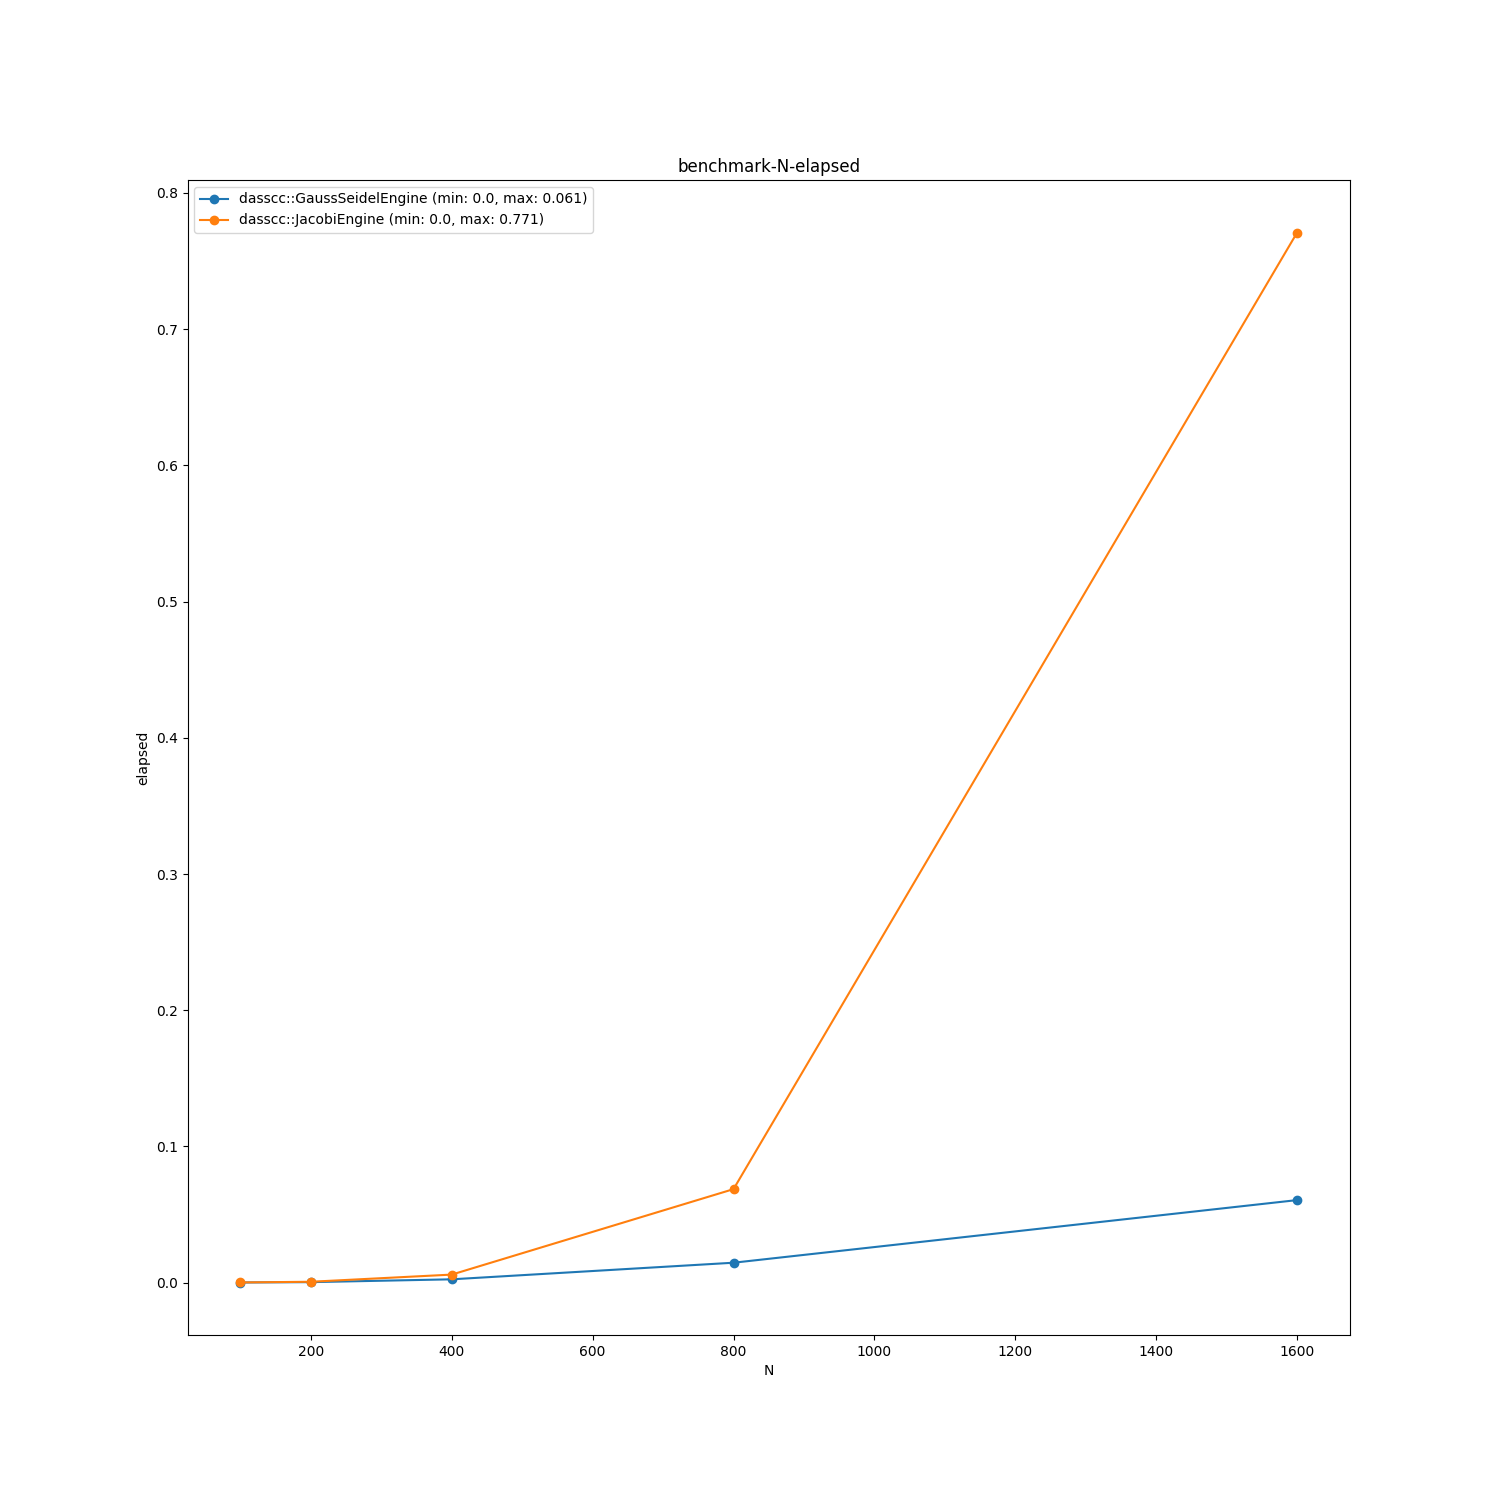
\includegraphics[width=0.7\linewidth]{images/001-benchmark-N-elapsed.png}
\end{figure}
\end{frame}

\begin{frame}
\frametitle{Scalabilit\`a - Dimensione - SPD}
\begin{figure}
  \centering
  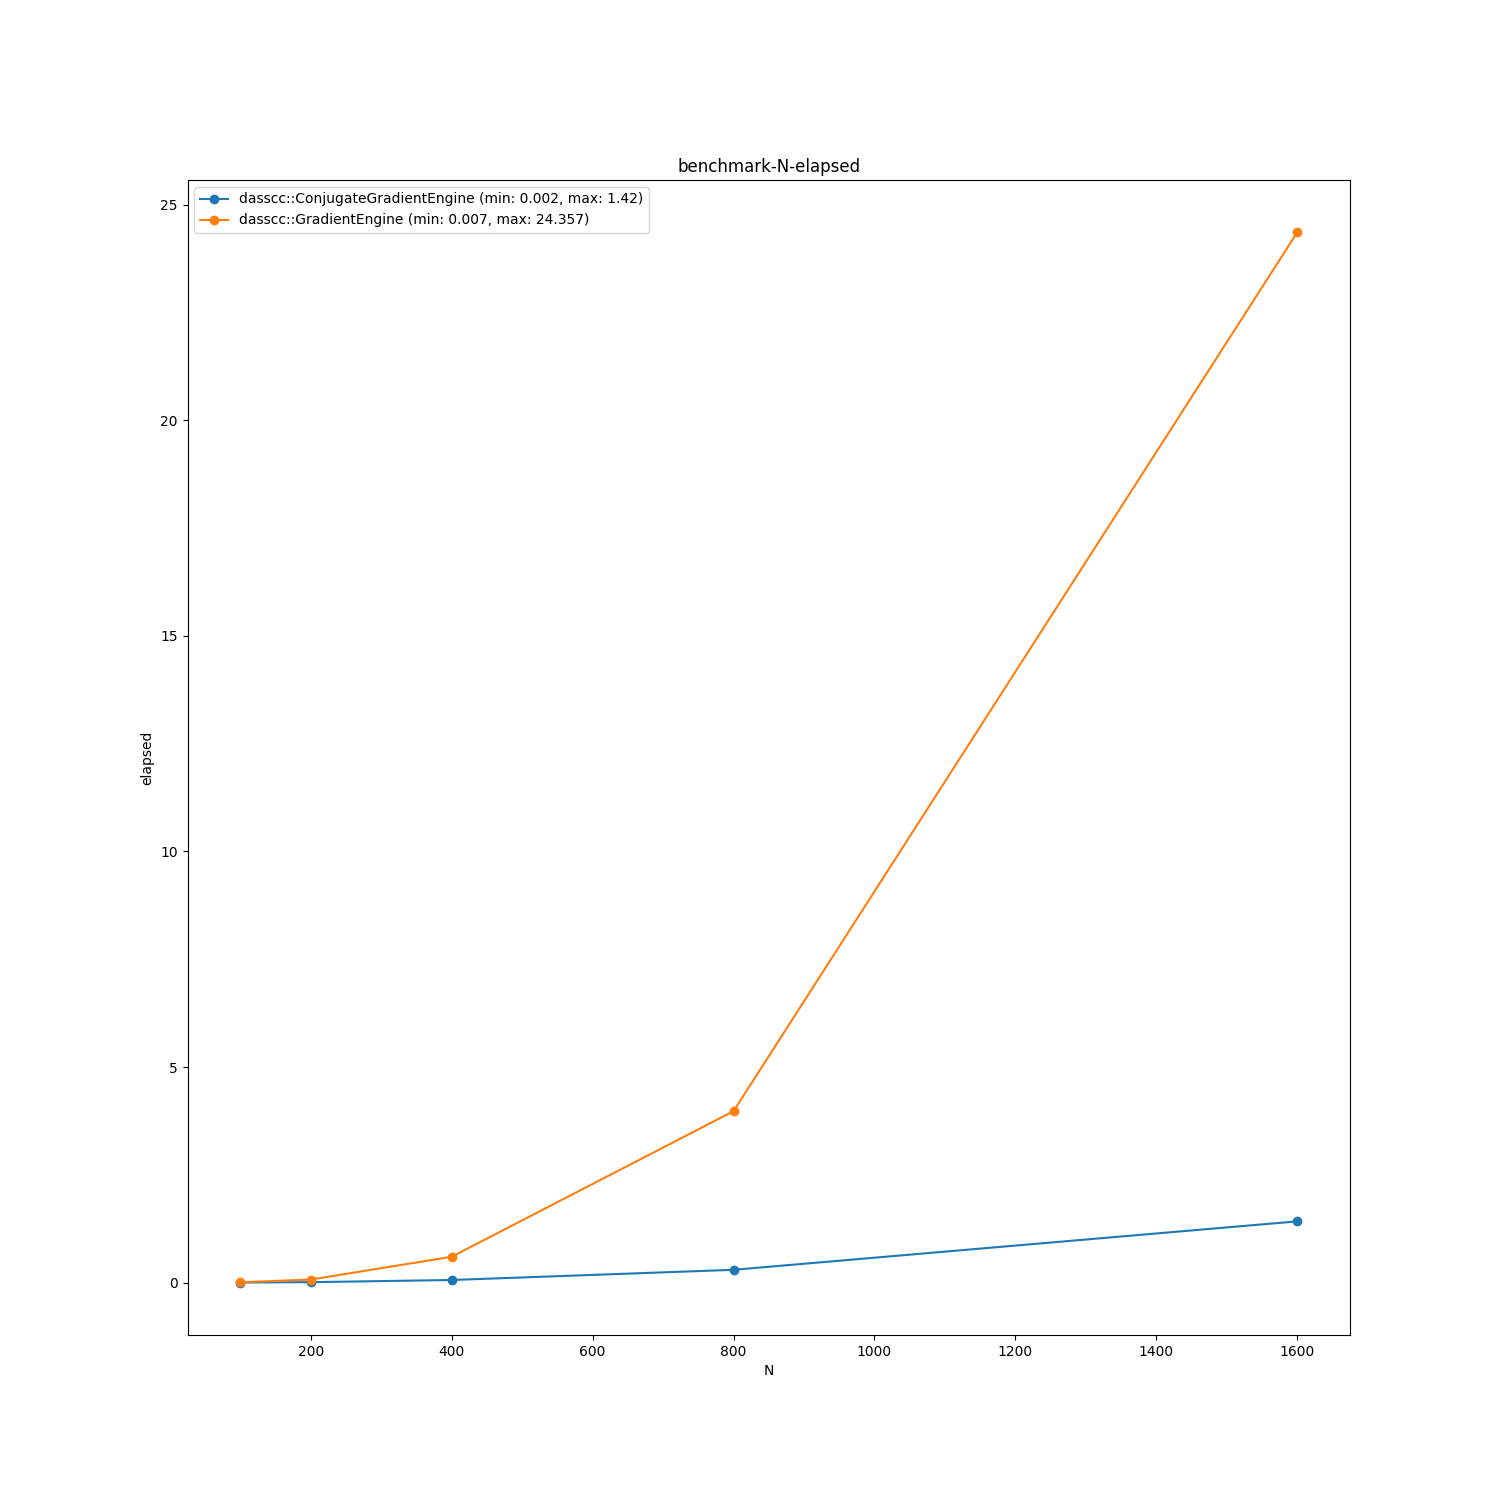
\includegraphics[width=0.7\linewidth]{images/002-benchmark-N-elapsed.png}
\end{figure}
\end{frame}

\begin{frame}
\frametitle{Scalabilit\`a - Densit\`a - RDD}
\begin{figure}
  \centering
  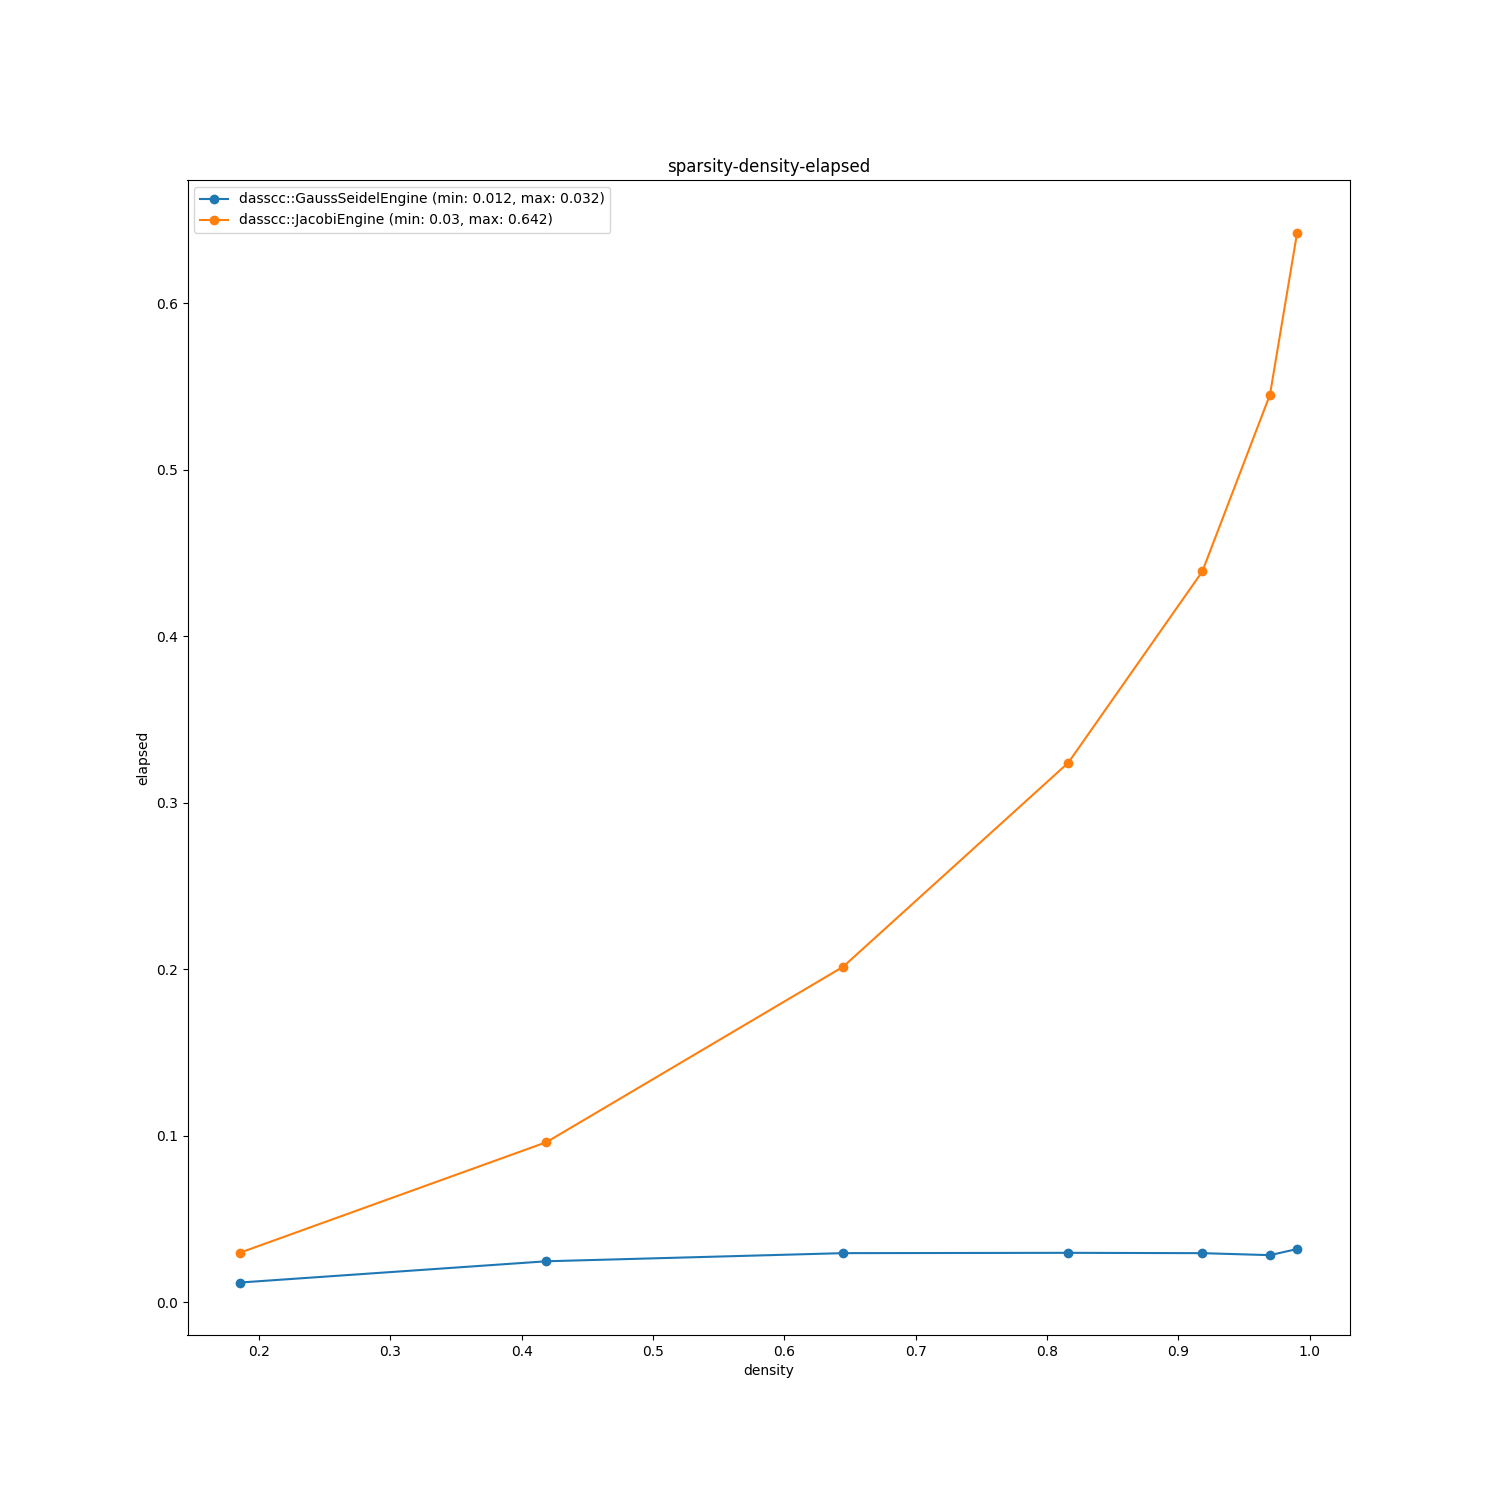
\includegraphics[width=0.7\linewidth]{images/001-sparsity-density-elapsed.png}
\end{figure}
\end{frame}

\begin{frame}
\frametitle{Scalabilit\`a - Densit\`a - SPD}
\begin{figure}
  \centering
  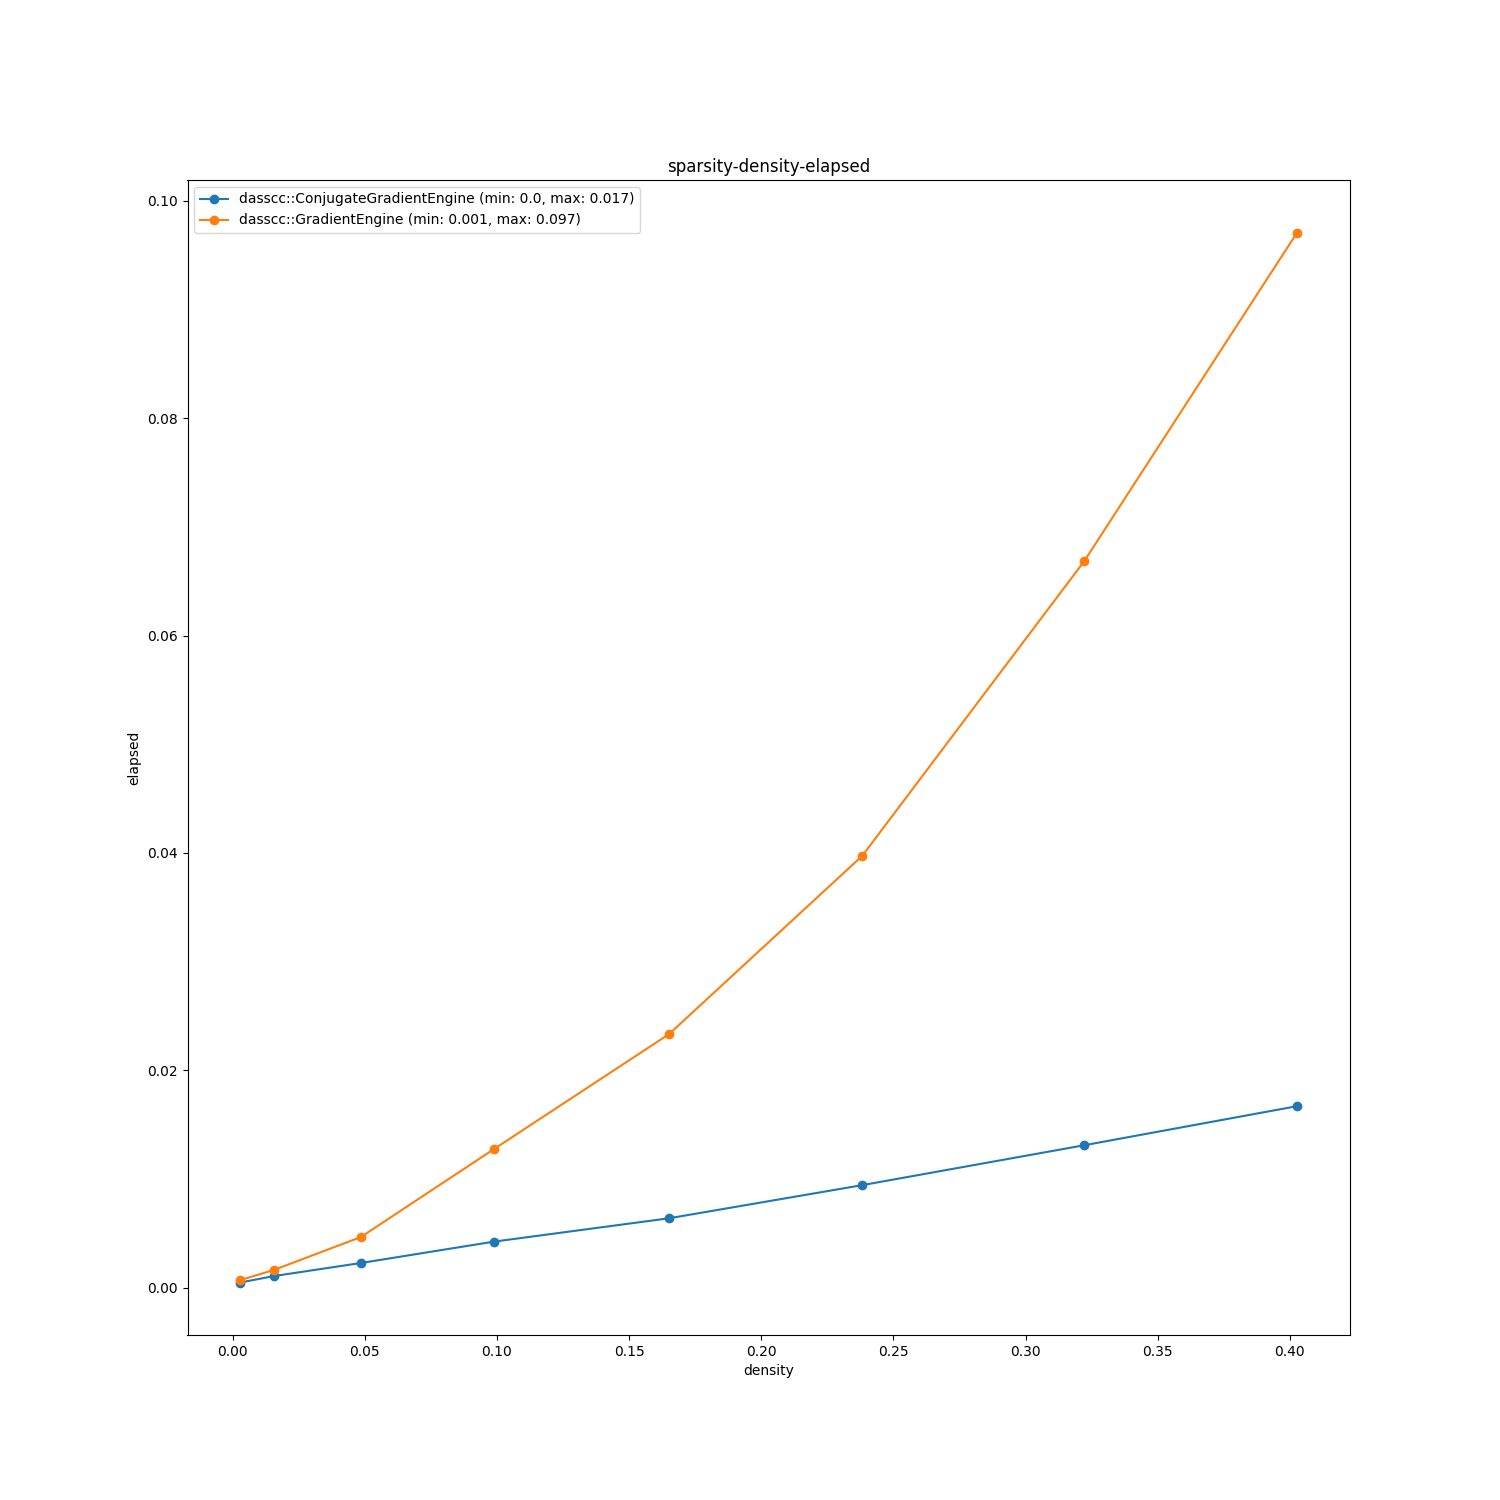
\includegraphics[width=0.7\linewidth]{images/002-sparsity-density-elapsed.png}
\end{figure}
\end{frame}

\begin{frame}
\centering
\Huge
Fine
\end{frame}

\end{document}
